\chapter{Objectives}

The goal of this project is the development and test of a low-cost electrical conductivity meter for liquids to be used as an aid to measure and analyze the flow in a photobioreactor.

The method chosen beforehand was to measure the fluids electrical conductivity, which can be changed easily by adding water with differing salt concentrations. Commercially available conductivity meters are built to measure with high accuracy in order to obtain information about a liquids absolute salinity and are relatively expensive. Our use case however does not need to create high accuracy absolute measurements, but measure a relative change allowing to distinguish two different liquids by their salinity. However, this needs to happen very fast and at a lot of different points in the stream. The more positions measured, the more complete the picture of the flow becomes. Therefore, the cost per sensor has to be low, to not put a restraint on the total number of points that can be measured.

The actual flow analysis is not part of this work, but rather the creation of a tool to make it possible. As such, the system needs to be designed to be used by others, not the creator himself. This thesis therefore describes a product development process rather than a scientific study. \\

The following sections describe and detail the requirements the sensor system has to fulfill in order to meet the objectives. These requirements translate the objectives into discrete and verifiable units, serving as the base for development and benchmark for the later performance analysis. 

\section{Spacial and Time Resolution}

The spacial and time resolution decide the granularity of the flow image.

The velocity $ v $ of the stream flowing over the sensor is approximately \unitfrac[1]{m}{s}. This allows us to create a relation \eqref{eq:resv} between the spacial resolution $ \diff s $ and the time resolution $ \diff t $.

\begin{equation}
	v = \dfrac{\diff s}{\diff t}
\label{eq:resv} 
\end{equation}

For example, a spacial resolution of \unit[1]{cm} would require a time resolution of \unit[0.01]{s}. However, this assumes the size $ l $ of the sensor and the time $ \tau $ a measurement takes to be infinitesimal small, while in reality it is not. While the sensors measures, the flow continuous and instead of measuring the conductivity of a certain volume at a certain time, an average is measured. Figure \ref{fig:cv} visualizes this issue.

\begin{figure}
	\begin{center}
		\begin{tikzpicture}
		\node [minimum height=32pt, minimum width=32pt, style=rect] (0) at (0, 0) {};
		\draw (-0.55,0) -- (-0.55,-1.5);
		\draw (0.55,0) -- (0.55,-1.5);
		\draw [darrow] (-0.55,-1.3) -- (0.55,-1.3) node[above, pos=0.5] {$l$};

		\node [minimum height=32pt, minimum width=32pt, style=vol] (0) at (-1.5, 0) {};
		\draw [arrow] (-2.05,1) -- (-1,1) node[above, pos=0.5] {$v$};

		\node [] at (4,0) {$t<0$};

		\node [minimum height=32pt, minimum width=32pt, style=rect] (0) at (0, -2.5) {};
		\node [minimum height=32pt, minimum width=32pt, style=vol] (0) at (-0.25, -2.5) {};

		\node [] at (4,-2.5) {$t=0$};

		\node [minimum height=32pt, minimum width=32pt, style=rect] (0) at (0, -4) {};
		\node [minimum height=32pt, minimum width=32pt, style=vol] (0) at (0.25, -4) {};

		\node [] at (4,-4) {$t=\tau$};		
		
		\node [minimum height=32pt, minimum width=32pt, style=rect] (0) at (0, -6) {};
		\node [minimum height=32pt, minimum width=32pt, style=vol] (0) at (1.5, -6) {};
		
		\node [] at (4,-6) {$t>\tau$};
		\end{tikzpicture}
		%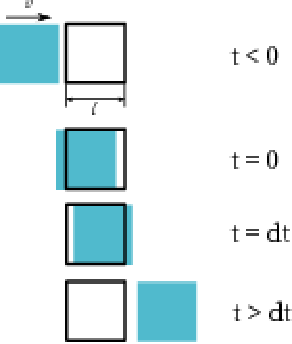
\includegraphics[width=0.45\textwidth]{images/resolution.pdf} 
		\caption{control volume moving over sensor}
		\label{fig:cv}
	\end{center}
\end{figure}

To accommodate for that, factors $ n $ \eqref{eq:resn} and $ k $ \eqref{eq:resk} are introduced, describing the ratio of the resolutions to the actual sizes.

\begin{equation}
	n = \dfrac{l}{\diff s}
\label{eq:resn} 
\end{equation}

\begin{equation}
	k = \dfrac{ \tau}{\diff t}
\label{eq:resk}
\end{equation}

Inserting $ k $ and $ n $ in formula \eqref{eq:resv} yields

\begin{equation}
	v = \dfrac{\diff s}{\diff t} = \dfrac{k \cdot l}{n \cdot \tau}
\label{eq:resv1} 
\end{equation}

The ratio $ r $
\begin{equation}
	r = \frac{k}{n}
\label{eq:resr} 
\end{equation}
is the ratio of the time it takes a control volume to enter and leave the sensor area  to the time a measurement takes. To avoid a smearing of the measurement over multiple control volumes, $ r $ should be 10. This can be achieved with a sensor that has a size $ l $ of \unit[1]{cm}, and a measurement time $ \tau $ of \unit[1]{ms}.

\section{Electrical Conductivity Resolution}

To measure the arrival of the new water stream after switching the water feed, the system has to be able to distinguish between water with different salinity. The water used normally in the reactor is tap water with a salinity of about \unit[0.2]{\%}. The salinity of the added saltwater can be chosen freely. Water with a salinity of about \unit[5]{\%} is easily available in the facilities and overs a sensible choice. Assuming a reactor with \unit[65]{l} in circulation and an added saltwater impulse of \unit[5]{l}, the resulting salinity after perfect homogenization would be approximately \unit[0.5]{\%}. The system has to be able to clearly distinguish between all those salinities.

\section{Cost}

The more sensors used, the more points in the stream can be measured and the better the image of the stream gets. Therefore, the cost per sensor has to be low enough to not be prohibitive of adding more sensors.

\section{Usability}

The sensor system is meant to be used in the algae reactors of the algae cultivation center at the Ludwig Bölkow Campus. It has to be possible to easily mount and remove the system to and from the reactor without having to dismantle it.

The system also has to be easy to use, so it can be helpful to the researchers working on the reactor. It has to work reliably and act according to expectations of the users. The chance of handling errors that lead to loss of data has to be minimized. All operations have to be documented in a minimal set of written instructions, so the system can still be used even if the designer isn't available anymore.

\begin{table}[H]
    \centering

    \caption[Requirements]{Requirements}
    \label{tab:req}
    \begin{tabular}{lp{.7\textwidth}l}
        	\toprule
        	Nr. & Requirement & Verification \tabularnewline
        	\midrule
		1 & The system shall have a time resolution of \unit[10]{ms}. & Test \tabularnewline
		2 & The system shall have a spacial resolution of \unit[1]{cm}. & Inspection \tabularnewline
		3 & The system shall cost less than \euro{10} per sensor.  & Analysis \tabularnewline
		4 & The system shall be deployable in the algae reactor. & Demonstr. \tabularnewline
		5 & The system shall be able to distinguish liquids with a difference in salinity of \unit[1]{\%}.  & Test \tabularnewline
		6 & The system shall be easy to use by anybody with only a minimal set of written instructions. & Test, Review \tabularnewline
        \bottomrule
    \end{tabular}
\end{table}